\documentclass[a4paper]{article}

\usepackage[english]{babel}
\usepackage[utf8]{inputenc}
\usepackage{amsmath}
\usepackage{graphicx}
\usepackage[colorinlistoftodos]{todonotes}
\usepackage{listings}

\title{\bf{Source Panel Method}}

\author{Utkarsh Chauhan}

\date{September 12, 2016}

\begin{document}
\maketitle

\section{Introduction}
\label{sec:introduction}

Source Panel Method is numerical technique of solving flow over any arbitrary shaped body by breaking its whole surface into finite sources sheets. Strength per unit length of the source is defined as {$\lambda$ = $\lambda$(s)}. Potential due to any small section \textit{ds} at point \textit{$($x,y$)$} will be given by

\begin{equation*}
    d\phi = \frac{\lambda ds}{2 \pi}\ln r
\end{equation*}
\newline
Now potential due to a sheet of source of length l at a point \textit{$($x,y$)$} will be given by

\begin{equation*}
    \phi \textit{$($x,y$)$} = \int_0^l\frac{\lambda ds}{2 \pi}\ln r
\end{equation*}
\newline
By the same logic is we divide a body into \textit{n} panels. The potential due to all \textit{j\textsuperscript{th}} panels on \textit{i\textsuperscript{th}} panel will be 

\begin{equation*}
    \phi \textit{$($x\textsubscript{i},y\textsubscript{i}$)$} = \sum_{j=1}^{n} \frac{\lambda_j}{2 \pi} \int_0^l\ln r_{ij} ds
\end{equation*}
\newline
where \textit{r\textsubscript{ij}} is the distance between \textit{i\textsuperscript{th}} and \textit{j\textsuperscript{th}} panel.\\
\newline
The normal component of velocity by a source is be given as 

\begin{equation*}
V_n = \frac{\partial }{\partial n_i}[\phi \textit{$($x\textsubscript{i},y\textsubscript{i}$)$}]
\end{equation*}
\newline
Applying the above \textit{Eq\textsuperscript{n}} for all the panels will give the total velocity at \textit{i\textsuperscript{th}} panel 

\begin{equation*}
V_n = \frac{\lambda_i}{2\pi} +  \sum_{j=1}^{n} \frac{\lambda_j}{2 \pi} \int_0^l \frac{\partial }{\partial n_i}(\ln r_{ij}) ds + V_\infty\cos\beta_i
\end{equation*}
\newline
as a boundary condition 
\begin{equation*}
V_n = 0
\end{equation*}
\pagebreak
\newline
By the same technique tangential velocity can be written as a sum of freestream velocity and induced velocities by the panels

\begin{equation*}
V_i = \frac{\lambda_i}{2\pi} +  \sum_{j=1}^{n} \frac{\lambda_j}{2 \pi} \int_0^l \frac{\partial }{\partial s}(\ln r_{ij}) ds + V_\infty\sin\beta_i
\end{equation*}
\newline
Now the pressure coefficient can be written in term of tangential velocity as 

\begin{equation*}
C_{p,i} = 1 - \left(\frac{V_i}{V_\infty}\right)^2
\end{equation*}
\newline
In order to calculate \textit{C\textsubscript{L}} and \textit{C\textsubscript{D}} the following formulas are used:
\begin{equation*}
C_L = - \frac{\sum_{i} C_{p,i}L_i\sin\beta_i}{b}
\end{equation*}
\begin{equation*}
C_D = \frac{\sum_{i} C_{p,i}L_i\cos\beta_i}{b}
\end{equation*}
\section{Source Panel Method for Ellipse}
\label{sec:example}

We will be appling the same method for calculating \textit{C\textsubscript{p}} distribution for an inverted ellipse with Major Axis = 10cm and Minor Axis = 5cm.
\newline
No. of Panels \textit{n} = 23
\newline
Velocity of freestream \textit{V\textsubscript{$\infty$}} = 23
\newline
The \textit{C\textsubscript{p}} distribution is calculated for 3 Angle of Attacks $\alpha$ = \textit{30\textsuperscript{o}}, \textit{60\textsuperscript{o}}, \textit{-34\textsuperscript{o}}
\newline
Given below is the MATLAB Code to generate the 

\lstinputlisting{Final.m}
\pagebreak
\section{Plots}
\label{sec:plots}
The following \textit{C\textsubscript{p}} distribution are obtained from the above Code
\newline
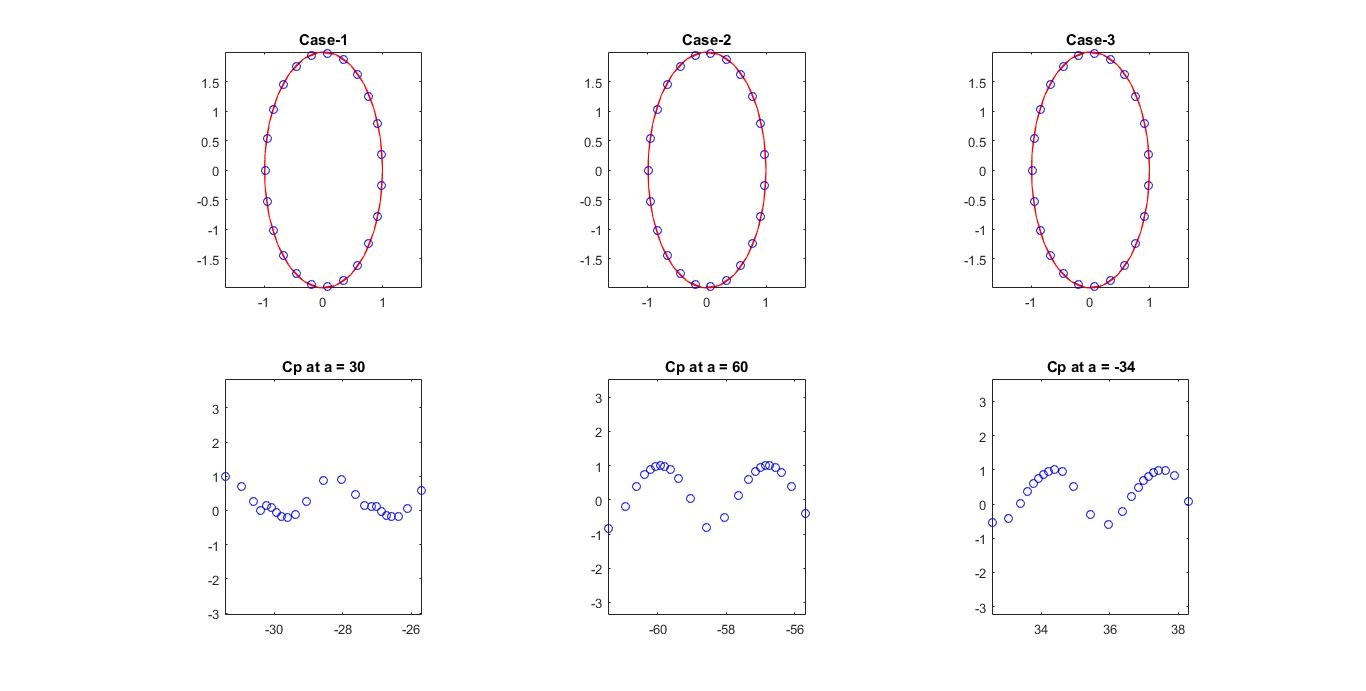
\includegraphics[scale=0.3]{Plots.jpg}
\newline
The Values of \textit{C\textsubscript{L}} and \textit{C\textsubscript{D}} are :
\newline
Value of \textit{C\textsubscript{L}} in Case 1 is 1.121745E-02
\newline
Value of \textit{C\textsubscript{D}} in Case 1 is -2.995293E-03 
\newline
Value of \textit{C\textsubscript{L}} in Case 2 is 6.246845E-03 
\newline
Value of \textit{C\textsubscript{D}} in Case 2 is 6.687941E-03
\newline
Value of \textit{C\textsubscript{L}} in Case 3 is 1.410285E-03
\newline
Value of \textit{C\textsubscript{D}} in Case 3 is -6.600087E-04 
\newline
\section{Conclusion}
\label{sec:Conclusion}
The above Plots gives a decent variation of \textit{C\textsubscript{p}} just with 23 Panels. It also shows that assuming the surface as a linear source is fairly nice approximation of the flow. In order to get even better distribution we can increase the no. of panels which will give us an even better result. More appropriate distribution can be obtained by interpolating points in between the given 23 points. At higher Velocities the method is not so reliable as the edges of panels are not smooth which will create disturbance in the flow.    


\pagebreak

\begin{thebibliography}{9}
\bibitem{1}
  John D. Anderson, Jr.
  \emph{Fundamentals of Aerodynamics}
  McGraw Hill Education (India) Private Limited
\bibitem{2}
  Some MATLAB Code Reference is taken from Source Panel Method 
  applied to Flow around Cylinder by Bilal Siddiqui
\end{thebibliography}
\end{document}
